\chapter{Infrastructure Automation and Cloud Deployment}
\label{sec:deployment}

While Chapter 4 detailed the software engineering and implementation of the Smart Travel application, writing source code represents only a fraction of the modern software delivery lifecycle. In a distributed environment comprising multiple independent backend services, external API gateways, message brokers, and isolated databases, manual testing, configuration, and deployment are no longer viable. 

This chapter details the transition of the Smart Travel platform from an isolated codebase to a live, scalable, and resilient cloud-native application. It first explores the foundational DevOps culture that drives modern software delivery. Subsequently, it details the implementation of a Continuous Integration and Continuous Delivery (\gls{CI/CD}) pipeline using Jenkins. Finally, it provides a comprehensive overview of how the platform's workloads are containerized, configured, and orchestrated within an OKD cluster.

%%%%%%%%%%%%%%%%%%%%%%%%%%%%%%
%%% 5.1 The DevOps Culture %%%
%%%%%%%%%%%%%%%%%%%%%%%%%%%%%%

\section{The DevOps Culture}
\label{sec:devops_culture}

Historically, the software engineering industry operated with rigid silos separating Development (Dev) teams, responsible for writing new features, and IT Operations (Ops) teams, responsible for maintaining system stability. This paradigm inherently created a conflict of interest: developers were incentivized to push changes rapidly to meet business demands, while operations teams were incentivized to block or delay changes to prevent production outages \cite{atlassian_devops_culture}.

The advent of \textit{DevOps} represents a cultural and technical movement designed to resolve this conflict by breaking down these organizational silos. At its core, DevOps is the combination of cultural philosophies, practices, and tools that increases an organization's ability to deliver applications at high velocity \cite{aws_what_is_devops}. It relies heavily on a model of shared responsibility, often summarized by the philosophy "you build it, you run it." Rather than handing off unverified code to a separate department, developers take accountability for the entire lifecycle of their software, from the initial commit to production monitoring \cite{atlassian_devops_culture}. 

In the context of the Smart Travel platform, adopting a DevOps mindset was not merely a philosophical choice, but a strict technical necessity. Deploying a single monolithic application manually over a secure file transfer protocol is tedious but feasible. Conversely, a microservices architecture decomposes an application into suites of independently deployable services \cite{fowler_microservices}. Manually compiling, containerizing, networking, and deploying the Angular frontend, the API Gateway, the distinct Spring and Quarkus domain microservices, Debezium, RabbitMQ, and multiple isolated MongoDB databases is an operational impossibility. 

Consequently, the distributed architecture mandates that every code change must be automatically built, comprehensively tested, and seamlessly deployed. The combination of microservices and increased release frequency leads to significantly more deployments, which can only be managed safely through rigorous automation \cite{aws_what_is_devops}.

%%%%%%%%%%%%%%%%%%%%%%%%%%%%%%%%%%%%%%%%%
%%% 5.2 CI/CD Pipeline Implementation %%%
%%%%%%%%%%%%%%%%%%%%%%%%%%%%%%%%%%%%%%%%%

\section{CI/CD Pipeline Implementation}
\label{sec:ci_cd}

To implement the DevOps philosophies discussed in the previous section, the Smart Travel platform relies on a (\gls{CI/CD}) pipeline orchestrated by Jenkins. 

The underlying infrastructure — including Jenkins and the target OKD cluster — was provisioned on an Amazon Web Services (AWS) EC2 instance by the company's IT Operations team. To ensure strict security perimeters, this environment has been entirely isolated from the public internet and only accessible via a secure SSH connection through a bastion host. Operating within this predefined infrastructure, the development focus shifted entirely to automating the software delivery lifecycle: writing declarative deployment pipelines, defining container specifications, and orchestrating the workload.

As illustrated in Figure \ref{fig:jenkins_dashboard}, the monolithic application concept is entirely abandoned at the CI/CD level. Instead, every individual microservice and infrastructure component (e.g., frontend, bff, travel catalog, orders, notification) features its own independent Jenkins pipeline, allowing them to be built, versioned, and deployed completely autonomously.

\begin{figure}[H]
    \centering
    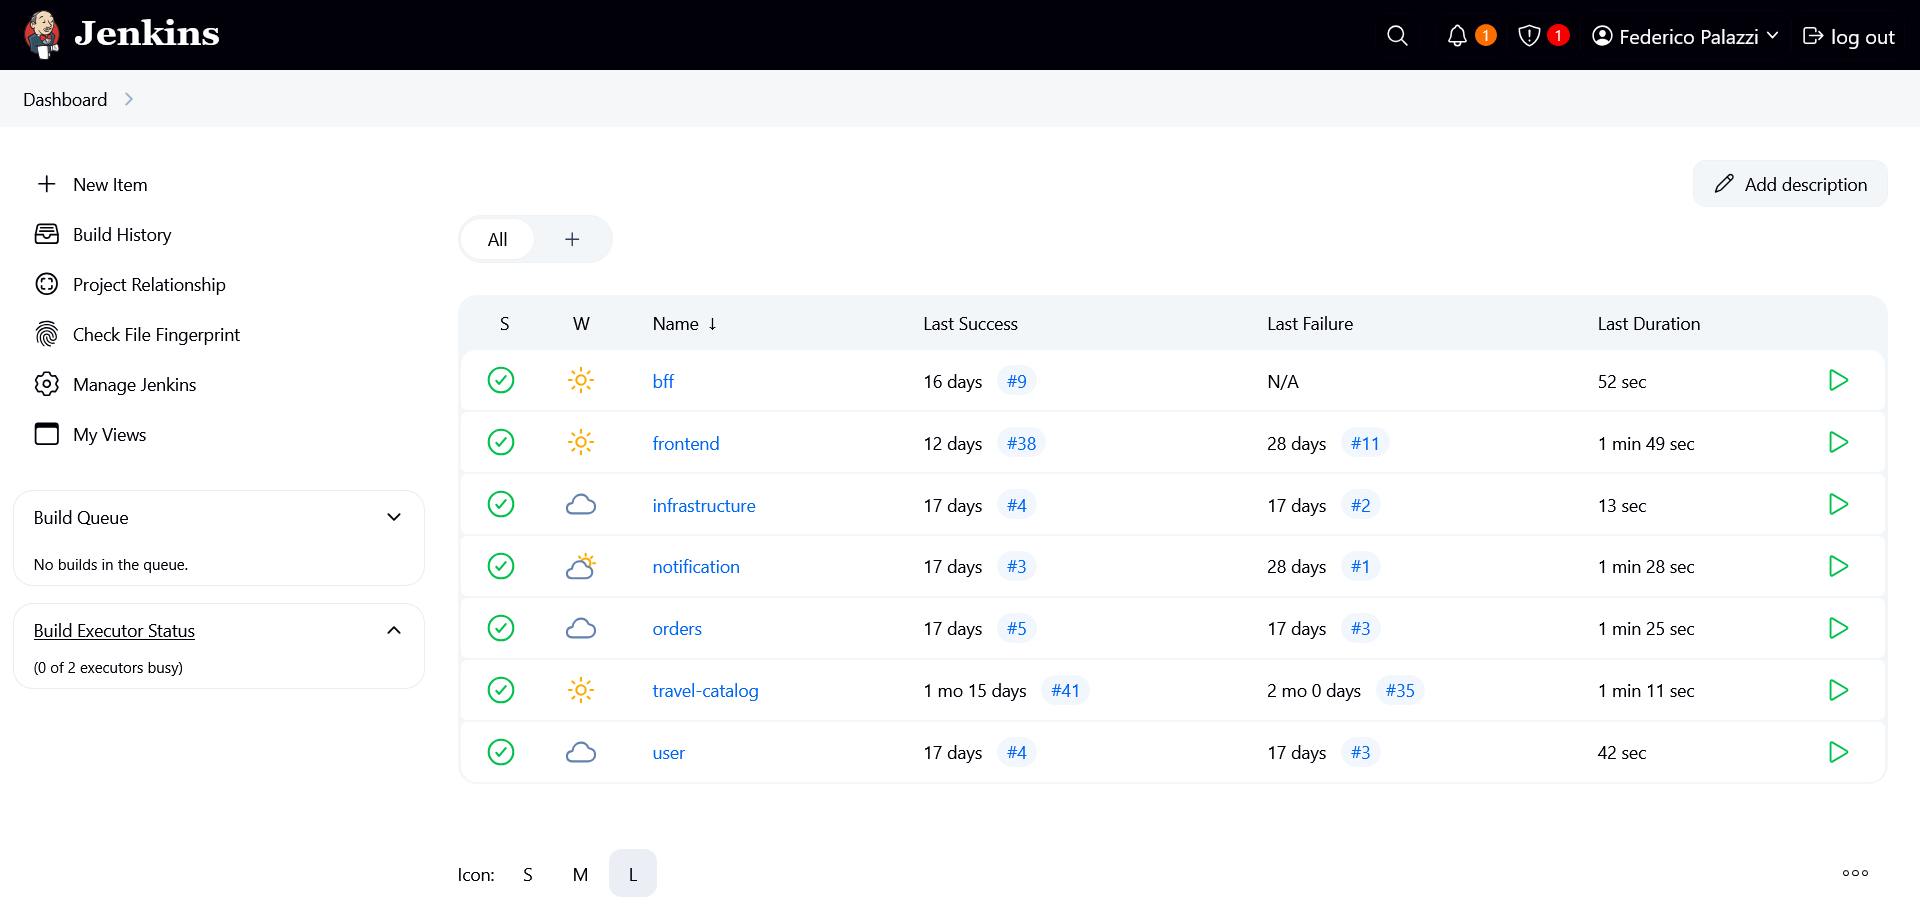
\includegraphics[width=\textwidth]{images/ch5/5_1_jenkins-dashboard.png}
    \caption[Jenkins CI/CD Dashboard]{The Jenkins Dashboard displaying the independent deployment pipelines for each microservice.}
    \label{fig:jenkins_dashboard}
\end{figure}

\subsection{Declarative Pipelines and Isolated Build Agents}

The deployment logic for each microservice is codified using Jenkins Declarative Pipelines (\texttt{Jenkinsfile}) stored directly alongside the application source code. A critical architectural choice in these pipelines is the use of isolated, ephemeral build agents via Docker.

Rather than installing Java, Maven, or Node.js directly onto the Jenkins host server — which often leads to version conflicts and "it works on my machine" anomalies — the pipelines instantiate specific Docker containers (for example, \texttt{maven:3.9.6-eclipse-temurin-21} for the backend and \texttt{node:20-alpine} for the frontend) to execute the build steps. This guarantees absolute reproducibility across all environments.

\begin{lstlisting}[language=Groovy, caption={Frontend Jenkinsfile: Isolated Node.js Build Agent}, label={lst:jenkins_frontend_build}]
stage('Build App') {
    agent {
        docker {
            image 'node:20-alpine'
            args '-u root'
        }
    }
    steps {
        script {
            // Dynamically extract version for Docker tagging
            def version = sh(
              script: "node -p require('./package.json').version",
              returnStdout: true
            ).trim()
            env.IMAGE_TAG = version
        }
        sh '''
          npm ci
          npm run build
        '''
    }
}
\end{lstlisting}

\subsection{Dependency Resolution and Dynamic Tagging}

For the Java microservices (such as the BFF and Notification API), the pipeline must resolve a complex dependency graph before compilation. Because the architecture relies on a \textit{common} module for shared DTO and interfaces (ensuring strict API contracts between services), the Jenkins pipeline implements a \texttt{Build Common} stage. 

As shown in the Jenkins console output (Figure \ref{fig:jenkins_console}), this stage securely checks out the shared repository using Git credentials and installs it into the ephemeral Maven \texttt{.m2} cache, allowing the subsequent application build to resolve the dependencies successfully.

\begin{figure}[H]
    \centering
    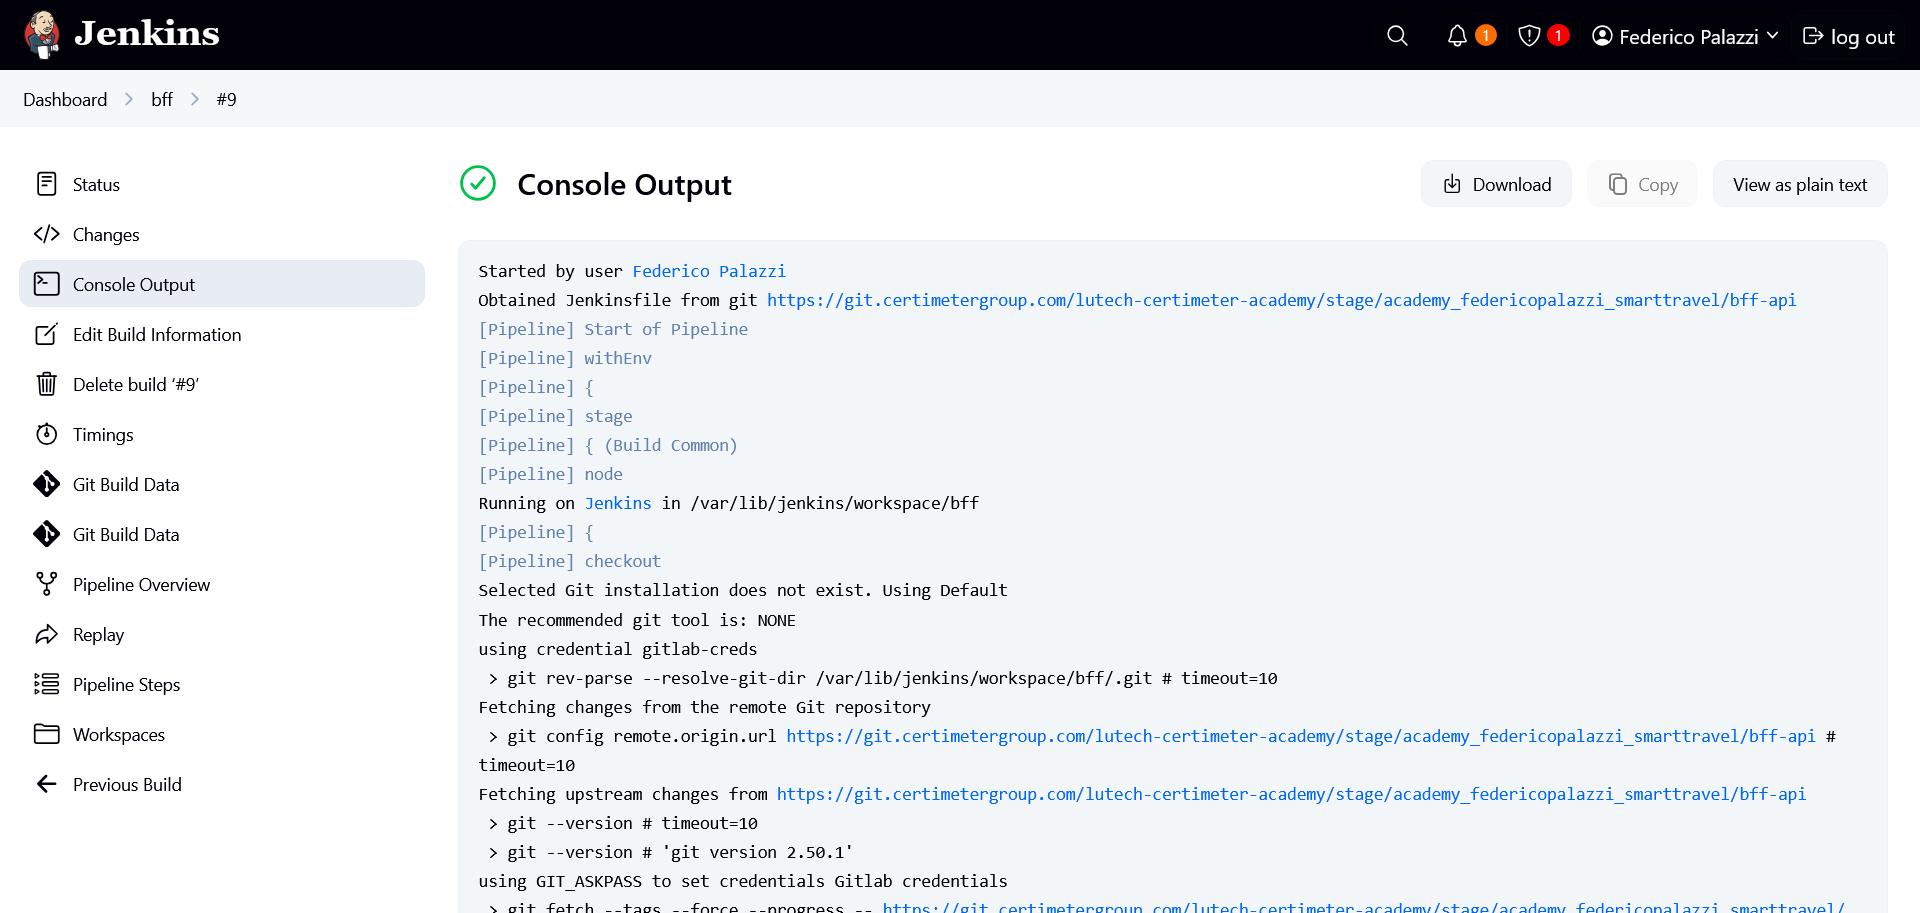
\includegraphics[width=\textwidth]{images/ch5/5_2_jenkins-console.png}
    \caption[Jenkins Pipeline Execution]{Console output of the BFF pipeline, demonstrating the successful execution of the \texttt{Build Common} declarative stage.}
    \label{fig:jenkins_console}
\end{figure}

Furthermore, the pipelines eliminate hardcoded versioning. Utilizing Groovy scripting, Jenkins dynamically interrogates the project's metadata files (\texttt{pom.xml} for Java, \texttt{package.json} for Angular) to extract the current semantic version. This version is directly injected into the pipeline's environment variables and used as the official tag for the Docker image, ensuring perfect alignment between the codebase version and the deployed container artifact.

\subsection{Containerization Strategy}

Once the application binaries are compiled, Jenkins triggers the containerization process. The Dockerfiles are strictly optimized for production. 

For the backend services, lightweight JRE (Java Runtime Environment) base images are utilized (\texttt{eclipse-temurin:21-jdk}). Notably, the Quarkus Notification API pipeline takes advantage of Quarkus's highly optimized \textit{uber-jar} packaging, avoiding the need for complex multi-stage Docker builds. For the Angular frontend, the compiled static assets are injected into an Nginx server image. The \texttt{Dockerfile} overrides the default Nginx configuration and adjusts directory permissions to allow execution under restricted security contexts.

\begin{lstlisting}[language=Dockerfile, caption={Angular Frontend Dockerfile}, label={lst:docker_frontend}]
FROM nginx:1.29

# Copy custom nginx config for SPA routing
COPY nginx.conf /etc/nginx/nginx.conf
COPY default.conf /etc/nginx/conf.d/default.conf

# Support running as arbitrary user for enhanced security
RUN chmod g+rwx /var/cache/nginx /var/run /var/log/nginx

# Copy built Angular app from Jenkins workspace
COPY dist/frontend/browser /usr/share/nginx/html

EXPOSE 8088
CMD ["nginx", "-g", "daemon off;"]
\end{lstlisting}

\subsection{Artifact Registry Publishing}

The final stage of the CI pipeline is publishing the immutable container image directly to the cluster's internal registry utilizing OKD \textit{ImageStreams}. Unlike traditional standalone container registries, an ImageStream provides an abstraction layer over container images from within the OKD cluster. This native integration is highly advantageous, as it allows OKD deployment configurations to automatically detect when a new image tag is pushed and immediately trigger a rolling update of the microservice.

To maintain security during this process, Jenkins utilizes the \texttt{withCredentials} plugin to inject the necessary registry authentication tokens directly into the execution context without exposing them in the console logs. 

The pipeline authenticates against the internal OKD registry, tags the newly built image with the dynamically extracted version and the designated cluster namespace, and pushes the artifact. Finally, it systematically cleans up the local Docker daemon cache to prevent storage exhaustion on the Jenkins build server. At this point, the artifact resides natively within the OKD environment, ready for container orchestration and workload distribution.

%%%%%%%%%%%%%%%%%%%%%%%%%%%%%%%%%%%%%%%%%%%%
%%% 5.3 Container orchestration with OKD %%%
%%%%%%%%%%%%%%%%%%%%%%%%%%%%%%%%%%%%%%%%%%%%

\section{Container Orchestration with OKD}
\label{sec:container_orchestration}

While Docker is excellent for packaging applications into immutable images, running a distributed microservices platform requires much more than simply starting containers. The system requires internal DNS resolution, load balancing, automated health checks, secure secret management, and self-healing capabilities (automatically restarting a crashed service). To achieve this, the industry relies on container orchestrators, specifically Kubernetes. 

The Smart Travel platform is deployed on an OKD cluster. A cluster is essentially a unified pool of compute resources (virtual machines known as worker nodes) managed by a central control plane. OKD, as the upstream community edition of Red Hat OpenShift, wraps standard Kubernetes with enterprise-grade security constraints, native \gls{CI/CD} pipelines, and enhanced developer dashboards.

\subsection{OKD Cluster Overview and Image Management}

The deployment lifecycle within OKD begins in the internal container registry. As discussed in Section \ref{sec:ci_cd}, the Jenkins pipeline pushes built artifacts directly to OKD \textit{ImageStreams} (Figure \ref{fig:okd_imagestreams}). An ImageStream is an OpenShift-specific resource that provides an abstraction layer over container images, allowing the cluster to centrally track image tags and metadata. 

While OKD ImageStreams possess the capability to automatically trigger rollouts upon detecting a new image, the Smart Travel platform intentionally implements a Continuous \textit{Delivery} model rather than automated Continuous \textit{Deployment}. Therefore, Jenkins is strictly responsible for building, tagging, and securely delivering the immutable artifacts to the cluster's registry. The actual rollout of the new application version is executed deliberately. This architectural decision ensures that administrators maintain strict, manual control over when infrastructure changes are applied to the live environment.

\begin{figure}[H]
    \centering
    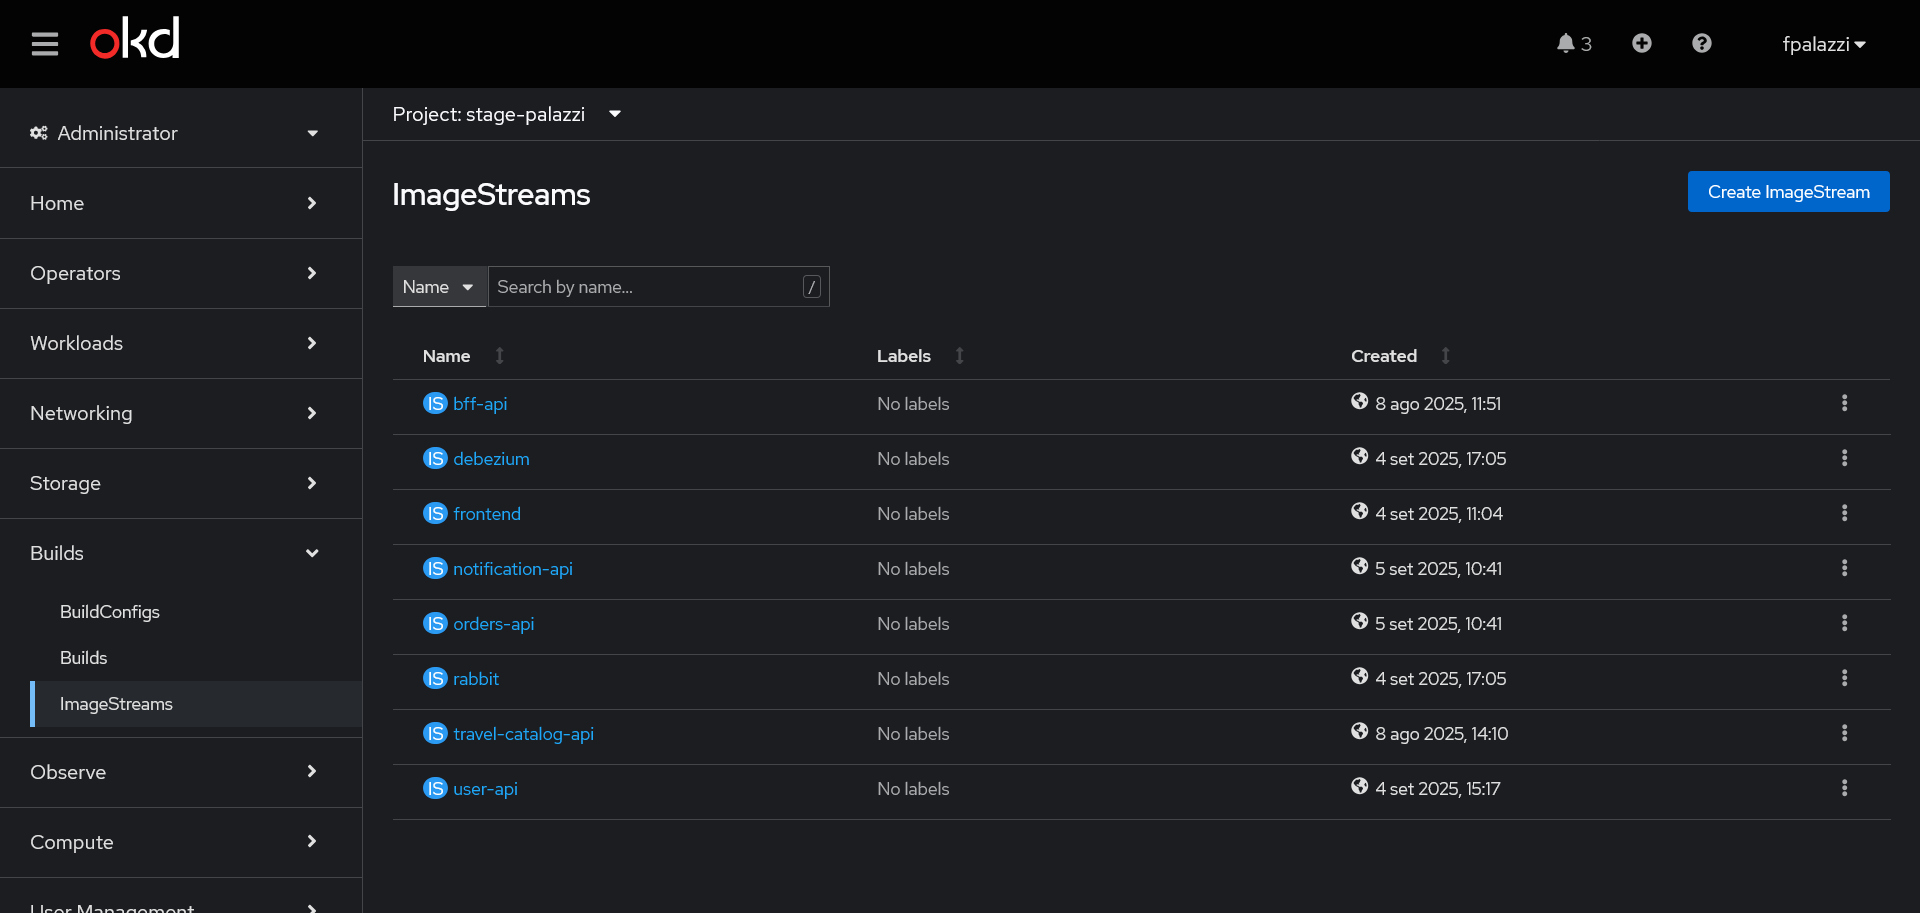
\includegraphics[width=\textwidth]{images/ch5/5_3_okd-imagestreams.png}
    \caption[OKD ImageStreams]{The OKD ImageStreams dashboard, demonstrating the internal tracking of the pushed container artifacts.}
    \label{fig:okd_imagestreams}
\end{figure}

Once the services are deployed, the OKD Topology view (Figure \ref{fig:okd_topology}) provides a visual representation of the application mesh, grouping interconnected pods, services, and routes.

\begin{figure}[H]
    \centering
    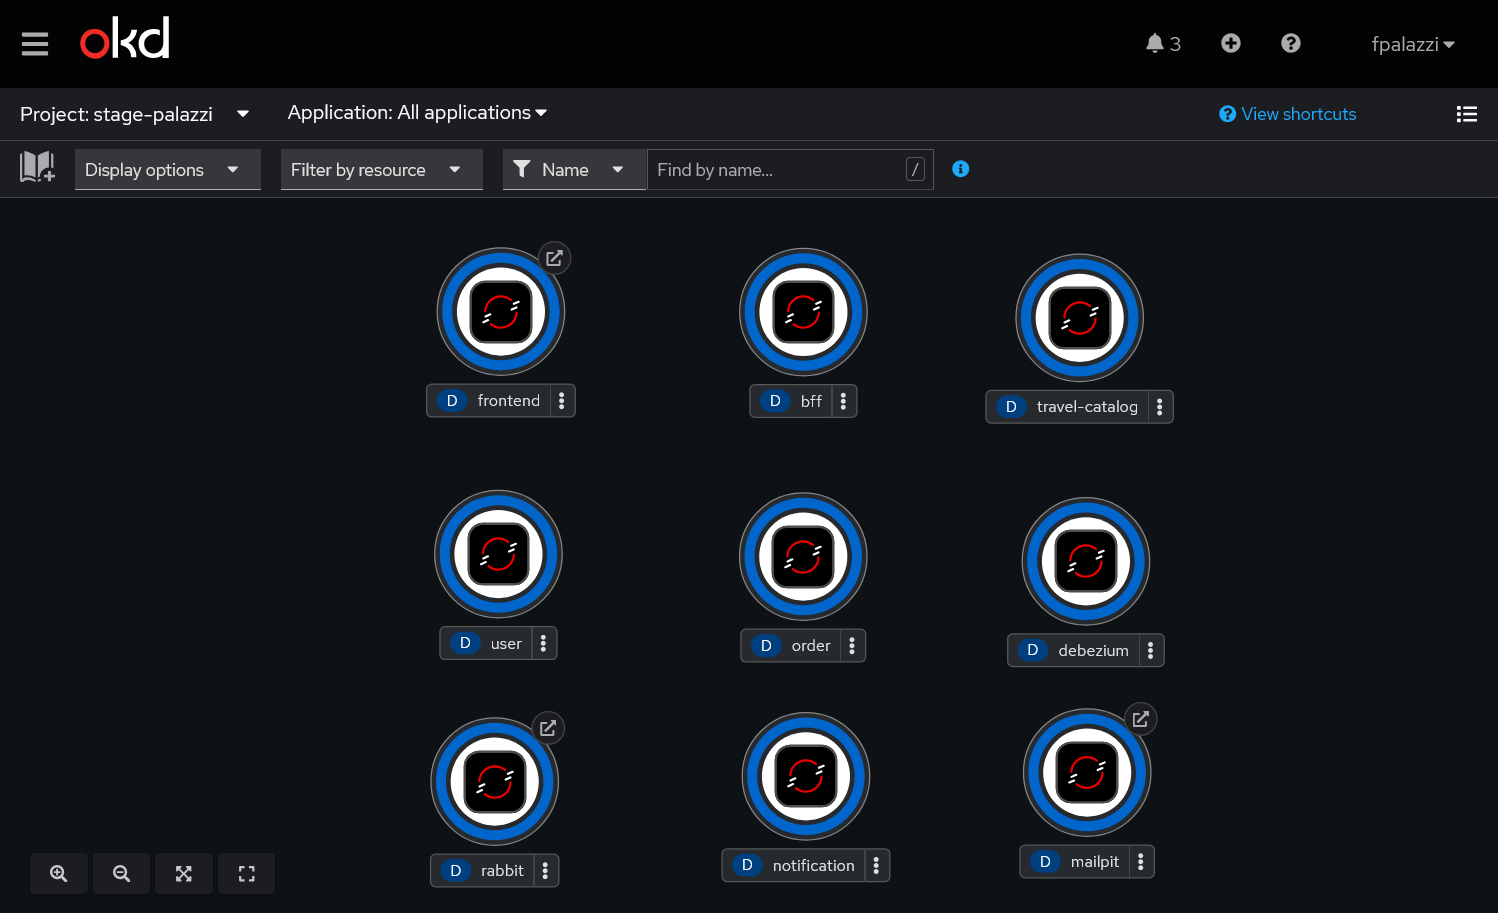
\includegraphics[width=0.9\textwidth]{images/ch5/5_4_okd-pods.png}
    \caption[OKD Topology View]{The visual topology of the Smart Travel cluster, illustrating the deployed microservices, message broker, and CDC components.}
    \label{fig:okd_topology}
\end{figure}

\subsection{Workload Management: Pods and Deployments}

In Kubernetes, the smallest deployable computing unit is a \textit{Pod}, which encapsulates one or more containers. However, Pods are ephemeral; if a node crashes, the Pod dies. To ensure high availability, the platform utilizes \texttt{Deployment} manifests. A Deployment acts as a declarative supervisor, ensuring that the specified number of container replicas is constantly running.

Because OKD enforces strict \textit{Security Context Constraints} (SCC), containers cannot run with root privileges by default. This required specific configurations in the deployment files. For example, the Angular frontend deployment explicitly disables privilege escalation and drops all root capabilities, ensuring the Nginx container executes securely.

\begin{lstlisting}[language=YAML, caption={Frontend Deployment Manifest Snippet}, label={lst:yaml_frontend_deployment}]
apiVersion: apps/v1
kind: Deployment
metadata:
  name: frontend
spec:
  replicas: 1
  template:
    spec:
      containers:
      - name: frontend
        image: image-registry.openshift-image-registry.svc:5000/stage-palazzi/frontend:0.0.14
        ports:
        - containerPort: 8088
        securityContext: # Required by OKD strict security constraints
          allowPrivilegeEscalation: false
          capabilities:
            drop:
              - ALL
          runAsNonRoot: true
\end{lstlisting}

\subsection{Configuration and Security: ConfigMaps and Secrets}

A core tenet of cloud-native development is the strict separation of code and configuration. To inject environment variables (such as downstream service URLs or database credentials) into the containers without hardcoding them in the source code, the deployment utilizes \texttt{ConfigMap} and \texttt{Secret} resources.

The \texttt{app-config} ConfigMap defines the internal cluster URLs used by the \gls{BFF} to communicate with the internal microservices. Conversely, sensitive data is stored as a base64-encoded \texttt{Secret}.

\begin{lstlisting}[language=YAML, caption={Cluster Configuration and Secret Resources}, label={lst:yaml_config_secret}]
apiVersion: v1
kind: ConfigMap
metadata:
  name: app-config
data:
  # Internal Kubernetes DNS names
  TRAVEL_CATALOG_URL: "http://travel-catalog-service:8080"
  ORDER_URL: "http://order-service:8082"
  BROKER_HOST: "rabbit-service"
---
apiVersion: v1
kind: Secret
metadata:
  name: app-secrets
type: Opaque
data:
  # Base64 encoded sensitive credentials
  PAYPAL_CLIENT_ID: QWJY... 
  PAYPAL_SECRET: RUZY...
\end{lstlisting}

These resources are dynamically injected into the deployed Pods via the \texttt{envFrom} directive in the deployment manifest, ensuring the containers remain entirely environment-agnostic.

\begin{figure}[H]
    \centering
    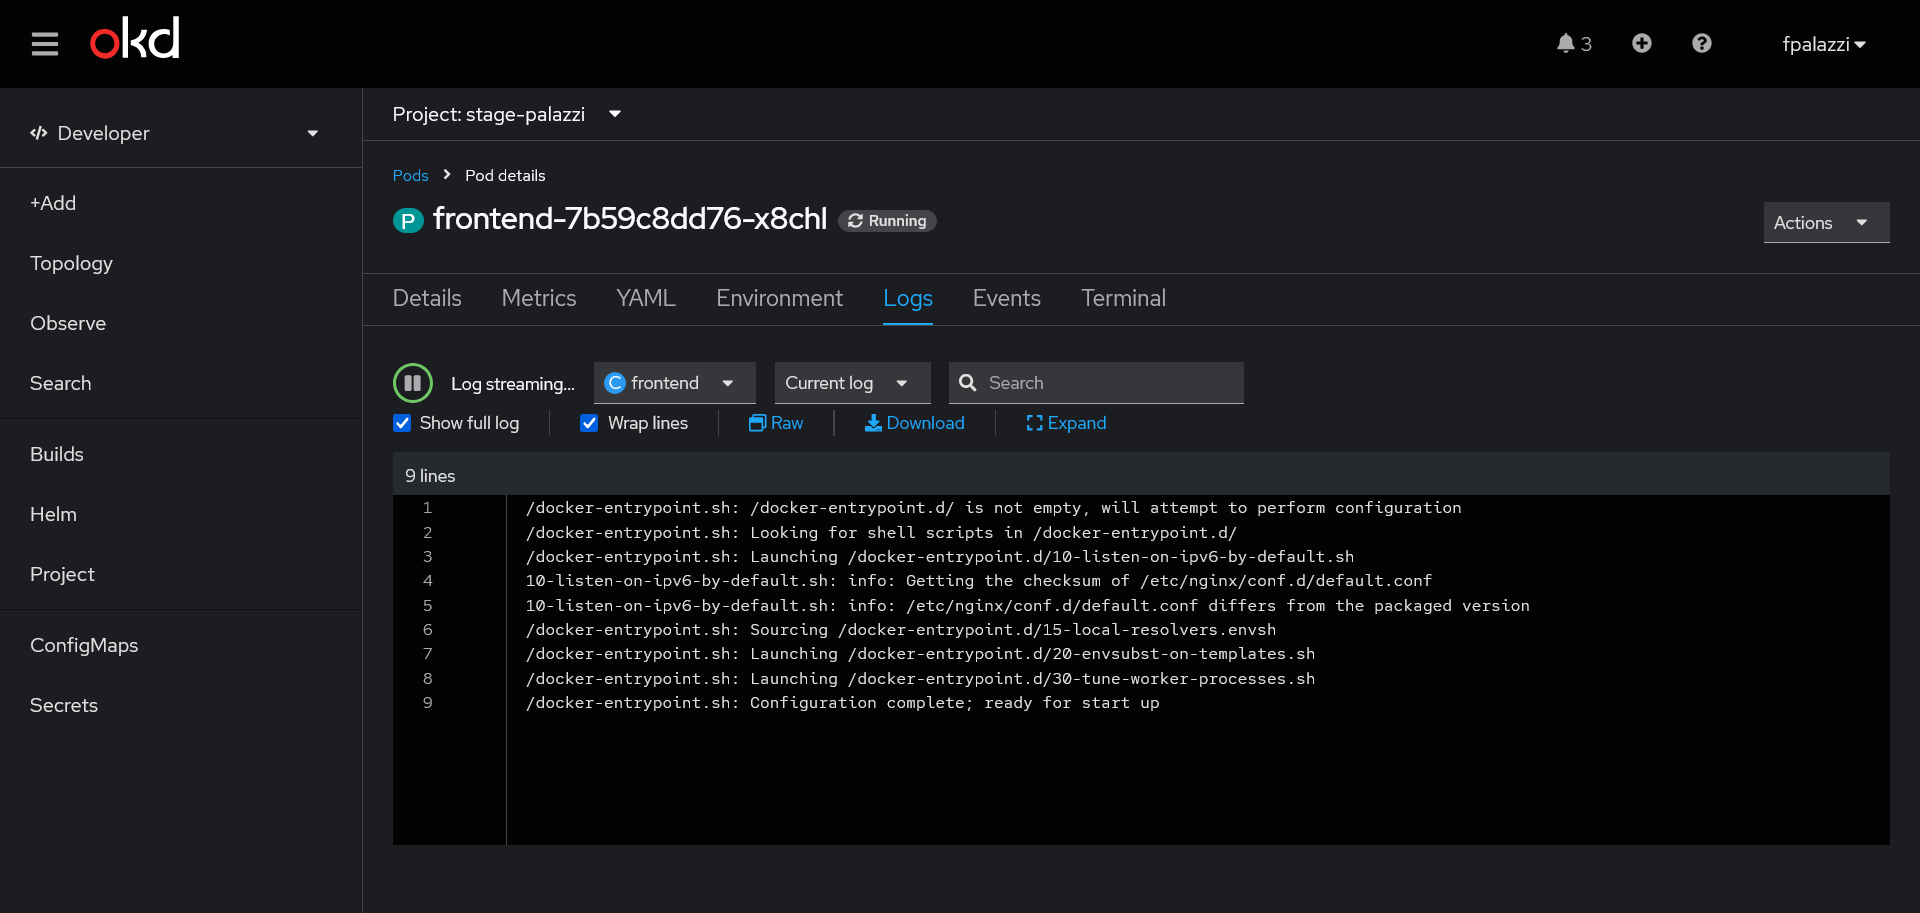
\includegraphics[width=\textwidth]{images/ch5/5_5_okd-pod-logs.png}
    \caption[Frontend Pod Logs]{OKD Pod Logs view confirming the successful, non-root initialization of the Nginx frontend container.}
    \label{fig:okd_pod_logs}
\end{figure}

\subsection{Networking: Services, Routes, and Reverse Proxying}

In a dynamic cluster, Pod IP addresses change constantly. To provide a stable networking interface, OKD uses the \texttt{Service} resource. A \texttt{Service} acts as an internal load balancer, creating a persistent internal IP and DNS record (e.g., \texttt{bff-service.stage-palazzi.svc.cluster.local}). 

However, \texttt{Services} are only accessible \textit{inside} the cluster. To expose an application to the public internet, we need to utilize a \texttt{Route} (an extended version of a Kubernetes Ingress), which provides edge termination for HTTPS and maps a public domain name to an internal service.

A critical architectural security decision was made regarding the \gls{BFF} API: \textbf{it does not possess a public Route}. To minimize the public attack surface, the BFF is completely isolated within the cluster. Instead, the public-facing Angular Frontend (running on Nginx) acts as a secure Reverse Proxy. 

The custom \texttt{nginx.conf} file is configured to intercept any incoming traffic targeting the \texttt{/graphql} or \texttt{/api/} paths. Using the internal OKD DNS resolver, Nginx securely forwards these requests directly to the hidden \texttt{bff-service}, preserving the original headers and passing through the authentication cookies while keeping the backend entirely shielded from direct external access.

\begin{lstlisting}[language=Nginx, caption={Nginx Reverse Proxy Configuration for the Hidden BFF}, label={lst:nginx_proxy}]
server {
    listen       8088;
    server_name  _;
    root   /usr/share/nginx/html;
    index  index.html;

    # Proxy GraphQL API calls to internal BFF service
    location /graphql {
        resolver 172.30.0.10 valid=30s; # DNS resolver - cluster DNS service IP
        # Route to the internal Kubernetes Service (not publicly exposed)
        set $upstream http://bff-service.stage-palazzi.svc.cluster.local:8085/graphql;
        proxy_pass         $upstream;
        proxy_http_version 1.1;
        # Pass through all authentication headers securely
        proxy_set_header   Authorization $http_authorization;
        proxy_set_header   Host $http_host;
        proxy_pass_request_headers on;
    }
    # Serve Angular SPA for all other routes
    location / { try_files $uri $uri/ /index.html; }
}
\end{lstlisting}

\begin{lstlisting}[language=YAML, caption={Frontend Service and Public Route Definition}, label={lst:yaml_frontend_route}]
apiVersion: v1
kind: Service
metadata:
  name: frontend-service
spec:
  selector:
    app: frontend
  ports:
    - port: 8088
      targetPort: 8088
  type: ClusterIP
---
apiVersion: route.openshift.io/v1
kind: Route
metadata:
  name: frontend-route
spec:
  host: smart-travel.apps.stage-soldi-okd.lutechstage.com
  to:
    kind: Service
    name: frontend-service
  tls:
    termination: edge
    insecureEdgeTerminationPolicy: Redirect
\end{lstlisting}
